%%%%%%%%%%%%%%%%%%%%%%%%%%%%%%%%%%%%%%%%
% Compact Laboratory Book
% LaTeX Template
% Version 1.0 (4/6/12)
%
% This template has been downloaded from:
% http://www.LaTeXTemplates.com
%
% Original author:
% Joan Queralt Gil (http://phobos.xtec.cat/jqueralt) using the labbook class by
% Frank Kuster (http://www.ctan.org/tex-archive/macros/latex/contrib/labbook/)
%
% License:
% CC BY-NC-SA 3.0 (http://creativecommons.org/licenses/by-nc-sa/3.0/)
%
% Important note:
% This template requires the labbook.cls file to be in the same directory as the
% .tex file. The labbook.cls file provides the necessary structure to create the
% lab book.
%
% The \lipsum[#] commands throughout this template generate dummy text
% to fill the template out. These commands should all be removed when 
% writing lab book content.
%
% HOW TO USE THIS TEMPLATE 
% Each day in the lab consists of three main things:
%
% 1. LABDAY: The first thing to put is the \labday{} command with a date in 
% curly brackets, this will make a new section showing that you are working
% on a new day.
%
% 2. EXPERIMENT/SUBEXPERIMENT: Next you need to specify what 
% experiment(s) and subexperiment(s) you are working on with a 
% \experiment{} and \subexperiment{} commands with the experiment 
% shorthand in the curly brackets. The experiment shorthand is defined in the 
% 'DEFINITION OF EXPERIMENTS' section below, this means you can 
% say \experiment{pcr} and the actual text written to the PDF will be what 
% you set the 'pcr' experiment to be. If the experiment is a one off, you can 
% just write it in the bracket without creating a shorthand. Note: if you don't 
% want to have an experiment, just leave this out and it won't be printed.
%
% 3. CONTENT: Following the experiment is the content, i.e. what progress 
% you made on the experiment that day.
%
%%%%%%%%%%%%%%%%%%%%%%%%%%%%%%%%%%%%%%%%%

%----------------------------------------------------------------------------------------
%	PACKAGES AND OTHER DOCUMENT CONFIGURATIONS
%----------------------------------------------------------------------------------------                               
%\UseRawInputEncoding
\documentclass[fontsize=11pt, % Document font size
                             paper=letter, % Document paper type
                             twoside, % Shifts odd pages to the left for easier reading when printed, can be changed to oneside
                             captions=tableheading,
                             index=totoc,
                             hyperref]{labbook}

%\documentclass[idxtotoc,hyperref,openany]{labbook} % 'openany' here removes the
   
\usepackage[bottom=10em]{geometry} % Reduces the whitespace at the bottom of the page so more text can fit

\usepackage[english]{babel} % English language
\usepackage{lipsum} % Used for inserting dummy 'Lorem ipsum' text into the template

\usepackage[utf8]{inputenc} % Uses the utf8 input encoding
\usepackage[T1]{fontenc} % Use 8-bit encoding that has 256 glyphs

\usepackage[osf]{mathpazo} % Palatino as the main font
\linespread{1.05}\selectfont % Palatino needs some extra spacing, here 5% extra
\usepackage[scaled=.88]{beramono} % Bera-Monospace
\usepackage[scaled=.86]{berasans} % Bera Sans-Serif

\usepackage{booktabs,array} % Packages for tables

\usepackage{amsmath} % For typesetting math
\usepackage{graphicx} % Required for including images
\usepackage{etoolbox}
\usepackage[norule]{footmisc} % Removes the horizontal rule from footnotes
\usepackage{lastpage} % Counts the number of pages of the document

\usepackage[dvipsnames]{xcolor}  % Allows the definition of hex colors
\usepackage{fancyvrb}
\definecolor{titleblue}{rgb}{0.16,0.24,0.64} % Custom color for the title on the title page
\definecolor{linkcolor}{rgb}{0,0,0.42} % Custom color for links - dark blue at the moment

\addtokomafont{title}{\Huge\color{titleblue}} % Titles in custom blue color
\addtokomafont{chapter}{\color{OliveGreen}} % Lab dates in olive green
\addtokomafont{section}{\color{Sepia}} % Sections in sepia
\addtokomafont{pagehead}{\normalfont\sffamily\color{gray}} % Header text in gray and sans serif
\addtokomafont{caption}{\footnotesize\itshape} % Small italic font size for captions
\addtokomafont{captionlabel}{\upshape\bfseries} % Bold for caption labels
\addtokomafont{descriptionlabel}{\rmfamily}
\setcapwidth[r]{10cm} % Right align caption text
\setkomafont{footnote}{\sffamily} % Footnotes in sans serif

\deffootnote[4cm]{4cm}{1em}{\textsuperscript{\thefootnotemark}} % Indent footnotes to line up with text

\DeclareFixedFont{\textcap}{T1}{phv}{bx}{n}{1.5cm} % Font for main title: Helvetica 1.5 cm
\DeclareFixedFont{\textaut}{T1}{phv}{bx}{n}{0.8cm} % Font for author name: Helvetica 0.8 cm

\usepackage[nouppercase,headsepline]{scrpage2} % Provides headers and footers configuration
\pagestyle{scrheadings} % Print the headers and footers on all pages
\clearscrheadfoot % Clean old definitions if they exist

\automark[chapter]{chapter}
\ohead{\headmark} % Prints outer header

\setlength{\headheight}{25pt} % Makes the header take up a bit of extra space for aesthetics
\setheadsepline{.4pt} % Creates a thin rule under the header
\addtokomafont{headsepline}{\color{lightgray}} % Colors the rule under the header light gray

\ofoot[\normalfont\normalcolor{\thepage\ |\  \pageref{LastPage}}]{\normalfont\normalcolor{\thepage\ |\  \pageref{LastPage}}} % Creates an outer footer of: "current page | total pages"

% These lines make it so each new lab day directly follows the previous one i.e. does not start on a new page - comment them out to separate lab days on new pages
\makeatletter
\patchcmd{\addchap}{\if@openright\cleardoublepage\else\clearpage\fi}{\par}{}{}
\makeatother
\renewcommand*{\chapterpagestyle}{scrheadings}

% These lines make it so every figure and equation in the document is numbered consecutively rather than restarting at 1 for each lab day - comment them out to remove this behavior
\usepackage{chngcntr}
\counterwithout{figure}{labday}
\counterwithout{equation}{labday}

% Hyperlink configuration
\usepackage[
    pdfauthor={}, % Your name for the author field in the PDF
    pdftitle={Laboratory Journal}, % PDF title
    pdfsubject={}, % PDF subject
    bookmarksopen=true,
    linktocpage=true,
    urlcolor=linkcolor, % Color of URLs
    citecolor=linkcolor, % Color of citations
    linkcolor=linkcolor, % Color of links to other pages/figures
    backref=page,
    pdfpagelabels=true,
    plainpages=false,
    colorlinks=true, % Turn off all coloring by changing this to false
    bookmarks=true,
    pdfview=FitB]{hyperref}

\usepackage[stretch=10]{microtype} % Slightly tweak font spacing for aesthetics
%\setlength\parindent{0pt} % Uncomment to remove all indentation from paragraphs

%----------------------------------------------------------------------------------------
%	DEFINITION OF EXPERIMENTS
%----------------------------------------------------------------------------------------

% Template: \newexperiment{<abbrev>}[<short form>]{<long form>}
% <abbrev> is the reference to use later in the .tex file in \experiment{}, the <short form> is only used in the table of contents and running title - it is optional, <long form> is what is printed in the lab book itself

\newexperiment{example}[Example experiment]{This is an example experiment}
\newexperiment{example2}[Example experiment 2]{This is another example experiment}
\newexperiment{example3}[Example experiment 3]{This is yet another example experiment}

\newsubexperiment{subexp_example}[Example sub-experiment]{This is an example sub-experiment}
\newsubexperiment{subexp_example2}[Example sub-experiment 2]{This is another example sub-experiment}
\newsubexperiment{subexp_example3}[Example sub-experiment 3]{This is yet another example sub-experiment}

%----------------------------------------------------------------------------------------
\newcommand{\HRule}{\rule{\linewidth}{0.5mm}} % Command to make the lines in the title page

\setlength\parindent{0pt} % Removes all indentation from paragraphs

\begin{document}

%----------------------------------------------------------------------------------------
%	TITLE PAGE
%----------------------------------------------------------------------------------------
%\frontmatter % Use Roman numerals for page numbers

%\begin{center}

%

\title{
\begin{center}
\href{http://www.bradley.edu}{
\includegraphics[height=0.5in]{figs/logoBU1-Print}}
\vskip10pt
\HRule \\[0.4cm]
{\Huge \bfseries Laboratory Notebook \\[0.5cm] \Large BEMOSS and Its Enhanced Applications}\\[0.4cm] % Degree
\HRule \\[1.5cm]
\end{center}
}
\author{\Huge Brian Lauer \\ \\ \LARGE blauer@mail.bradley.edu \\[2cm]} % Your name and email address
\date{Beginning March 13, 2018} % Beginning date
\maketitle

%\maketitle % Title page

\printindex
\tableofcontents % Table of contents
\newpage % Start lab look on a new page

\begin{addmargin}[0cm]{0cm} % Makes the text width much shorter for a compact look

\pagestyle{scrheadings} % Begin using headers

%----------------------------------------------------------------------------------------
%	LAB BOOK CONTENTS
%----------------------------------------------------------------------------------------
\labday{Monday, May 06, 2019}
I emailed Mr. Mattus asking him whether he made any progress on finding a laptop that
can be used to demonstrate the installation of BEMOSS. 
 
\labday{Thursday, May 09, 2019}
I picked up a department laptop from Mr. Mattus today. He cleared the partition
completely, so no time had to be spent removing a previous operating system from the
machine. Then, I installed Ubuntu 16.04.6 LTS on the system with a bootable USB flash
from the link provided on the BEMOSS installation guide.

\labday{Wednesday, May 22, 2019}
As recommended by Dr. Miah, I worked on running BEMOSS on the previous team’s laptop. By running \texttt{./startBEMOSS\_GUI.sh} inside the directory \texttt{/home/bemoss/BEMOSS3.5/GUI}, I was able to start up the BEMOSS Launcher Wizard. By selecting Run BEMOSS in the TKinter GUI the server was started,
and I was able to connect to the local web server at \texttt{localhost:8082.}. At this point, the software was able to detect the WeMo Insight Switch and thus control the Philips Hue bulb connected to it. I was not able to control the motor due to time constraints, but I will do so soon.
\medbreak\noindent
I did some more research on the features that BEMOSS offers at https://github.com/
bemoss/BEMOSS3.5/wiki/BEMOSS-Features including the ability to provide local and remote monitoring and security.

\labday{Thursday, May 23, 2019}

\labday{Friday, May 24, 2019}
The hierarchy of BEMOSS was researched today with the motivation of understanding
the software better in the Developer Resources. The first layer consists of the UI and User
Management which reside in the central server. Here admins can manage different nodes
on the network and either deny or accept requests from users. Layer 2 is the BEMOSS
Application and Data Management Layer which allows developers to create custom
applications for target devices that can be added to the UI. It may be interesting to explore
this feature once I have gotten a better idea of what sort of original contributions I would
like to make to the project. A motivation for this part of BEMOSS is to integrate web
services like IFTTT (IF This Then That) which may be interesting to use. The third layer is
the operating system and framework layer consisting of the agent platform VOLTTRON
developed by the Pacific Northwest National Laboratory. Six different agents perform
various different tasks such as detecting new devices (lighting/plug load controllers)
on the network and monitoring them to ensure they are running properly. Layer 4 is
the BEMOSS connectivity layer that handles the communication between the operating
system layer and the physical hardware devices. This is where support is extended
to different communication technologies like Wi-Fi, Ethernet, and Serial(RS-485). Each
device supported by BEMOSS has an API translator needed to handle the differences in
device attributes.

\labday{Monday, May 27, 2019}
No work was done due to Memorial Day.

\labday{Tuesday, May 28, 2019}
The outline for the presentation on May 31 follows:
\begin{itemize}
\item Introduction
\item Applications of BEMOSS
\item Hardware/software needed to install BEMOSS
\item Immediate future work
\end{itemize}

The following questions are answered to determine what needs to be added to the
presentation:

\begin{itemize}
\item What is BEMOSS? BEMOSS or Building Energy Management Open Source Software
is an agent-based software platform engineered to allow small- and medium-sized
commercial buildings to more seamlessly integrate equipment designed for sensing
and control. This software can allow building owners and engineers to manage
building energy use better by monitoring different load control devices such as
lighting loads, plug loads, and HVAC controllers.
\item How can BEMOSS be applied to the real world?
\item What hardware and software is needed to install BEMOSS?
\item What kind of future work is available to be implemented with this software?
\end{itemize}

After working on the presentation, I worked in the lab to document the toggling of
the WeMo insight switch with BEMOSS. Most of this information was gathered from
https://github.com/bemoss/BEMOSS3.5/wiki/User-Guide-for-BEMOSS-UI.
Once the BEMOSS server has started, type localhost:8082 in the web browser to go to
the BEMOSS Web UI. The username is ’admin’ and the password is the one set during
installation. To discover the switch, click the "Discover New Devices" tab in the left
navigation bar. Under the "All Plug Load Controllers" menu, select either "All Plug Load
Controllers" or "Belkin International Inc. Insight." Click "Discover Selected Devices" to
complete the process. The number of discovered devices will appear on the Discover
New Devices tab. If only one device has been discovered, a 1 will appear next to the
name Discover/Manage. On the Discover/Manage page, approve the device by setting the
approval status to "Approved" then select "Save Changes to Plugload Controllers." Navigate to the tab NODE$1$. Select "View All" under "Plugload", then select the WeMo smart plug icon to change the status of the plug and view the power consumption.  

\labday{Wednesday, May 29, 2019}
I spent the first few hours of the day reading through \cite{Pipattanasomporn2015}. I worked on researching the applications of BEMOSS and the introduction for the May 31st presentation. The future work still needs to be researched and added. Also, I would like to add some pictures to the slides to help the audience members gain a better visual understanding. Ideally, the presentation should be finished tomorrow morning, so I can have more time to practice. I practiced the presentation at the end of the day today without everything completed which isolated my knowledge gaps and gave me a better idea of what I should work on. To provide better flow between slides I must find ways to transition well between them. 

\labday{Thursday, May 30, 2019}
More work was done on the presentation.

\labday{Friday, May 31, 2019}
Work on presentation and meeting with other members of the Robotics and Mechatronics (RAM) group.

\labday{Monday, June 3, 2019}
I read through \cite{Zhang2016} and \cite{Khan2018} to obtain more ideas on original contributions I can make to the project. One thing I found in \cite{Khan2018} is the use of an induction motor in McNeese State University's microgrid. With a variable frequency drive, this could be integrated with BEMOSS to control different types of industrial loads. One problem is the high price tag on both. In \cite{Zhang2016}, a Particle Photon board was used to control the brightness of fluorescent lighting via step-dim ballasts. The Raspberry Pi is definitely a better option here than the Photon board as the previous senior project group used an RPi in their project. 

\labday{Tuesday, June 4, 2019}
Today, I attempted to install BEMOSS on my Ubuntu laptop. After running \texttt{./startBEMOSSGUI\_.sh} in the GUI directory, I encountered some problems. The following errors were thrown:
\begin{Verbatim}[tabsize=4]
Traceback (most recent call last):
	File "Web_Server/run/defaultDB.py", line 91, in <module>
		admin = User.objects.get(username='admin')
	File "/home/ramgroup/BEMOSS3.5/env/local/lib/python2.7/
	site-packages/django/db/models/manager.py", 
	line 85, in manager_method
		return getattr(self.get_queryset(), name)(*args, **kwargs)
	File "/home/ramgroup/BEMOSS3.5/env/local/lib/
	python2.7/site-packages/django/db/models/query.py", 
	line 379, in get
		self.model._meta.object._name
django.contrib.auth.models.DoesNotExist: User matching query does not exist.
OS settings imported
\end{Verbatim}

\begin{Verbatim}[tabsize=4]
Traceback (most recent call last):
	File "bemoss_lib/databases/cassandraAPI/initialize.py",line 186 in
<module>
		init()
	File "bemoss_lib/databases/cassandraAPI/initialize.py", line 99, in init
		casYamlFile = open(settings.PROJECT_DIR+"/cassandra/conf/cassandra.yaml",'r')
IOError: [Errno 2] No such file or directory: 
'/home/ramgroup/BEMOSS3.5/cassandra/conf/cassandra.yaml'
\end{Verbatim}

I was able to eliminate the first error by using 'admin' for the Django superuser rather than the default 'ramgroup'. I tried to eliminate the second error by deleting BEMOSS3.5 from my home directory and recloning; however, the same problem persisted. I found a directory named \texttt{~/BEMOSS3.5/cassandra} on the previous group's laptop which is not being created when I run BEMOSS on my machine. This directory contains the file "cassandra.yaml" which the file "initialize.py" is attempting to access. This leads me to believing that there is some issue with the creation of the directory.

\labday{Monday, June 10, 2019}
More work was done to install BEMOSS. I emailed one of the members of the previous senior project named Bob about the error.

\labday{Tuesday, June 11, 2019}
After looking through some of the files in \texttt{/BEMOSS3.5/GUI/GUI.py}, I found the line of code preventing the installation of BEMOSS which is 108:
\begin{verbatim}
bemoss_is_installed = os.path.isdir(ui_path) and os.path.isdir(cassandra_path) 
and os.path.isdir(env_path)
\end{verbatim}
Since the cassandra directory is non-existent, the expression \texttt{os.path.isdir(cassandra\_path)} evaluates as \texttt{False}.
\bigbreak\noindent
After some further searching I found that the BEMOSS is failing to download and install the cassandra database due to a dead link in the shell script
\begin{verbatim}
/BEMOSS3.5/GUI/bemoss_install_v3.5.sh
\end{verbatim} 
When line 48:
\begin{verbatim}
wget http://downloads.datastax.com/community/dsc-cassandra-3.0.9-bin.tar.gz
\end{verbatim} is run, a "404 not found" error is generated by the server. The URL was entered into a web browser and it was found that the requested URL was not found on the server.
\bigbreak\noindent
As a possible solution, I used a different URL to download the cassandra database in
\begin{verbatim}
/BEMOSS3.5/GUI/bemoss_install_v3.5.sh
\end{verbatim}
After adding a comment on line 48, the previously mentioned URL on line 49 is changed to
\begin{verbatim}
https://archive.apache.org/dist/cassandra/3.0.9/
apache-cassandra-3.0.9-bin.tar.gz
\end{verbatim}
Lines 49-53 were changed to
\begin{verbatim}
wget https://archive.apache.org/dist/cassandra/3.0.9/
apache-cassandra-3.0.9-bin.tar.gz
tar -xzf apache-cassandra-3.0.9-bin.tar.gz
sudo rm apache-cassandra-3.0.9-bin.tar.gz
sudo rm -rf cassandra/
sudo mv apache-cassandra-3.0.9 cassandra
\end{verbatim}  
After this, BEMOSS was successfully installed.
The post-installation instructions were followed on the BEMOSS wiki, but, at the end, errors were still being thrown while attempting to get the web server up and running.

\labday{Wednesday, June 12, 2019}
After viewing the issue on the BEMOSS repo:
\url{https://github.com/bemoss/BEMOSS3.5/issues/47}, I found that the IP address in \texttt{parent\_ip.txt} did not match the IP of my system, so I changed this to the correct IP. This corrected the problem and the BEMOSS web server was able to boot successfully. Note this text file is only created after BEMOSS is run.

\labday{Thursday, June 13, 2019}
In the lab, I worked on getting BEMOSS up and running. I mistakenly used the wired connection at first when attempting to run the BEMOSS server but decided to connect to the wireless network ECE-Robotics1 as the Raspberry Pi controlling the motor uses this network. I was able to login as admin into BEMOSS but experienced a problem when attempting to connect to the WeMo Insight switch. When I attempt to navigate to the plug load page to control the WeMo switch the page does not load. It is unclear whether this is an issue with the Insight switch or with BEMOSS itself. I also tried working with the WeMo plug on the previous group's Ubuntu laptop but ran into the same issue leading me to believe it is possibly an issue with the WeMo switch.

\labday{Friday, June 14, 2019}
More work was done at the beginning of the day to help identify and fix the problem of the Plugload page not loading. After one attempt the page eventually loaded but took a great deal of time. It was finally discovered that the laptop must be connected to the wired network as well as ECE-Robotics1 in order to function properly. Without a wired connection, the PC is unable to connect to the Internet which causes errors. However, although the software was working properly errors were reported by the TSDagent. These are captured in the figure below.
\bigbreak\noindent
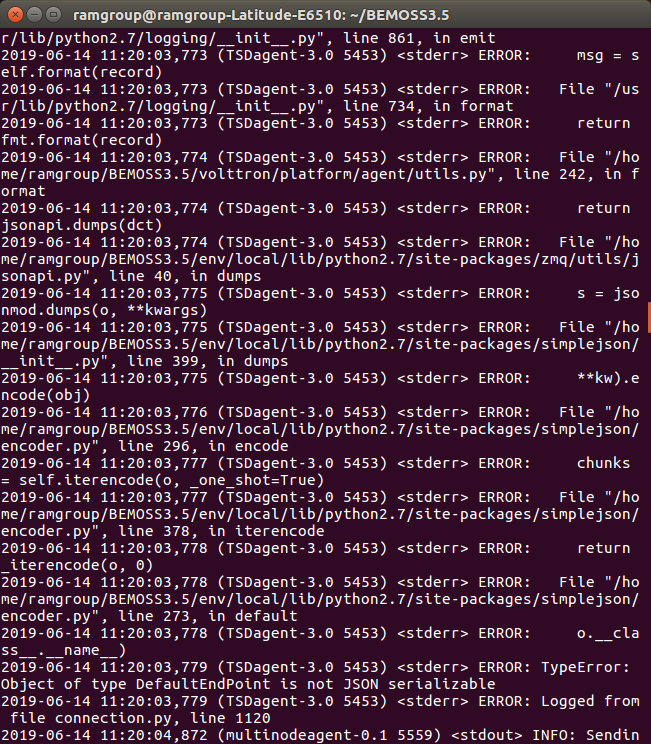
\includegraphics[scale=0.5]{figs/screenshot61419.png}

I decided to try the same setup on the previous group's machine to see if I would receive the same problem. After running the software on the previous group's machine, I received the same errors with the TSDagent thus concluding that the proposed solution mentioned on page 31 is not a complete one. I will need to email Ashraf with the details on this. 
\bigbreak\noindent
In the meantime, I will attempt to get the DC motor running with the BEMOSS software. After modifying the file permissions of three of \texttt{shell\_control.sh} using
\begin{verbatim}
chmod u+x shell_control.sh
\end{verbatim}
I was able to identify and control the motor using \texttt{pyshell\_control.py} which rotates the motor counter clockwise then clockwise. Soon I need to start creating the GUI that will show all devices on the network and enable the ability to control them.

\labday{Monday, June 17, 2019}
Work on the presentation slides for June 21 was done. Further research on the Beamer class was conducted to add more detail to the presentation.

\labday{Tuesday, June 18, 2019}
The presentation slides are almost complete at this point. A few more captions need to be added to the figures and sources must be added to the bibliography.

\labday{Wednesday, June 19, 2019}
Work on the presentation was continued and uploaded to github. A few additions may need to be made as I was not able to get a full 10 minutes out of it. Tonight, the presentation will be practiced  and polished, so that I am ready to go by Friday. This time I need to know exactly what I am saying before going in so I can avoid any pauses.
\bigbreak\noindent
A page on wikipedia on computer networks was read:
\begin{verbatim}
https://en.wikipedia.org/wiki/Computer_network
\end{verbatim}
to better understand what is going on with this project. Knowledge of the python Tk interface must be obtained to build the GUI due June 21.


\labday{Thursday, June 20, 2019}
Had a short meeting with Dr. Miah in the lab. Here is what needs to be done:
\begin{itemize}
\item Add progress and plan to presentation.
\item IoT discovery and control GUI and BEMOSS plugload icon must be implemented before June 28. Conference paper must be completed and submitted before June 28. However, this is not likely to be finished by then as little to no progress has been made on the GUI or BEMOSS motor integration.
\item Need to start recording hours when working with the DC motor so I can get paid. I need to talk with Mrs. Polen to get an account setup with Bradley. 
\item I need to start thinking of a device to implement in BEMOSS. Otherwise, this project will not be successful without an original contribution. Thus, a lot of research must be done.
\item Agent-based architecture will need to be researched by reading some research papers.
\item Need to send Ashraf an email asking if he has made any progress on the project.
\bigbreak\noindent
All the scripts written by Reece and Bob to control the motor were understood except for \texttt{XBEETEST.py} on the Raspberry Pi as I still need to do research on the XBee modules if I am to use them in the project.
\end{itemize}

\labday{Friday, June 21, 2019}
To better understand how to create the GUI to control the devices in the lab, I read up on the documentation for PyGTK at \url{https://python-gtk-3-tutorial.readthedocs.io/en/latest/layout.html#}. 

\labday{Sunday, June 23, 2019}
Work was done on researching a device to integrate within BEMOSS. Here are some possible ideas:
\begin{itemize}
\item Ultrasonic Range Finding module - hcsr$04$\\
I have one of these and have been programming it some and could potentially have an interesting application for IoT. However, this does seem rather simple and would not likely take long to fully implement.
\item Digital Multimeter
\item Accelerometer
\item Gyroscope
\item Dust Sensor \url{https://www.waveshare.com/dust-sensor.htm}
\item PM2.5 Particle Sensor \url{https://www.cytron.io/p-honeywell-pm2.5-particle-sensor-module} Looking at this module it uses a two wire UART output so it would likely be very easy to interface with the Raspberry Pi 
\end{itemize}

\labday{Monday, June 24, 2019}
While building the GUI, I came to realize that Gtk is simply too complex for me, so I decided to change tkinter which is a bit simpler. At this point I have finished the GUI and simply need to connect the callbacks to the events using tk.widget.bind(event,callback). Once this has been done I will be ready to move on to implementing the logic to control the wemo switch and motor within the tkinter application.

\labday{Tuesday, June 25, 2019}
To better understand lower level networking concepts, I will use the python module \texttt{socket} to ping addresses on the network and resolve their hostnames. It may save time to use the \texttt{nmap} command used by the previous group; however, I would like to build a system from scratch completely in python. As the motor needs to be implemented within BEMOSS as soon as possible, I will work on this first and determine how to use the wemo switch later. I will base some of my work off \cite{scanopy}. However, after working for some time I found that the program I was attempting to write was rather inefficient and using the nmap command will be much more faster. Thus I have decided to use the scripts written by Bob and Reece. I was able to write a single python script using the socket module to parse through all hosts on the network 'ECE-Robotics$1$' and place them in a list along with their respective IP addresses.

\labday{Wednesday, June 26, 2019}
I was able to succesfully add the Raspberry Pi and Wemo switch names to the listbox; however if the button 'Discover IoT Devices' is pressed continually, devices will continually be added to the list. Right now I need to determine how to initialize the Raspberry Pi by sshing into it. Then, after selecting the toogle button, I must figure out how to remotely send commands to the device to turn it on or off without having to reconnect. After some tinkering I found that I can simply just ssh into the pi and run a script that simply turns the moltor on when the button is toggled on and off when the button is toggled off. Thus no initializatin will be needed. 
\bigbreak\noindent
I need to write scripts to perform the following operations:
\begin{itemize}
\item Use nmap to the scan wifi credentials
\item Place the credentials into text file
\item Scan for the IP addresses and place them into a text file
\item Assign the address read from the file to a variable and use this to remotely login to the device (for the RPi)
\end{itemize}
However, I have almost no knowledge of bash so this will take some researching. I found a way of storing the first IP address in \texttt{IPAddresses.txt} in a variable that can be used to call the python scripts running on the pi to control the motor. Each time the toggle button is pressed, the text file is read from which is inefficient. More ideally I would like to implement some feature where the IP addresses of the devices are stored in a place that can be accessible to any shell script within the directory. I would like to do this later on; however, I need to move on to working the Wemo switch's API into this application.
\bigbreak\noindent
To perform the implementation of the WeMo switch, I will need to read through the documentation provided by the BEMOSS team and some of the python code to find exactly what code needs to be written to create a fully functional system. This code is very complicated thus it may take a great deal of time to work through.
\bigbreak\noindent
I found a url on the bemoss website: \url{www.bemoss.org/api-interface-wemo-smart-plug/} that explains how some of the code works. The switch uses the upnp (Universal Plug and Play) protocol. 

\labday{Thursday, June 27, 2019}
A github gist was located that contains a script to control a wemo device: \url{https://gist.github.com/pruppert/af7d38cb7b7ca75584ef}. I was able to successfully control the wemo switch with this. This will be helpful in understanding the code provided in the bemoss repo and on the bemoss website. The url to send commands to the switch is

\begin{verbatim}
http://192.168.1.112:49153/upnp/control/basicevent1
\end{verbatim}
I attempted to add this url into the method \texttt{getDeviceStatus}; however when I run the code I receive a 500 response (internal server error). After running an nmap scan with the port scan enabled I found that the wemo switch uses both ports 53 and 49153 for communication, so the cause of the problem here is unknown. Later, I determined the problem is that no XML was being sent in the body of the POST request to the device. I simply copied the XML from the python script I found online to control the switch and modified the code from the bemoss website. This is the function used to turn on the Insight switch.
\begin{Verbatim}[tabsize=4]
def turnOnSwitch():
	header = {
		'Content-Type': 'text/xml; charset="utf-8"',
		'SOAPACTION': '"urn:Belkin:service:basicevent:1#SetBinaryState"'
	}
	body='<?xml version="1.0" encoding="utf-8"?>
<s:Envelope xmlns:s="http://schemas.xmlsoap.org/soap/envelope/" 
s:encodingStyle="http://schemas.xmlsoap.org/soap/encoding/">
<s:Body><u:SetBinaryState xmlns:u="urn:Belkin:service:basicevent:1">
<BinaryState>1</BinaryState>
</u:SetBinaryState></s:Body></s:Envelope>'
	controlUrl='http://192.168.1.112:49153/upnp/control/basicevent1'
	response = requests.post(controlUrl, body, headers=header)
	del response																																										
\end{Verbatim}
To understand how this code works more research will need to be done as I know very little about XML.

\labday{Friday, June 28, 2019}
Layer 1 (UI layer) of the BEMOSS hierarchy was researched for a few hours to try and understand how new devices are to be added to BEMOSS. Details such as how the 	Model-Message-View-Template works and the UI project structure are provided. However, this doesn't really provide any details on what happens when an element in the UI is selected such as pressing a button to toggle a device on and how the message flows down to the device. In other words, I'm not able to understand the chain between the UI layer and the device as this is not documented on the BEMOSS wiki. A single file I found that could be possibly helpful is \texttt{~/BEMOSS3.5/Web\_Server/webapps/device/templates/plugload/plugload.html}. This will require some digging to understand the html, css, and jQuery as I have little to no experience in any of these. In addition, I may need to research the agent based system to understand how these agents interact with the devices' APIs.   

\labday{Monday, July 1, 2019}
To understand how the device discovery agent works, I studied each line of 
\begin{verbatim}
BEMOSS3.5/Agents/DeviceDiscoveryAgent/devicediscovery/agent.py
\end{verbatim}
carefully. In \texttt{BEMOSS3.5/BEMOSS\_lib/db\_helper.py} a class named 
% Note using underscore by itself will throw an error as it is normally used to typeset underscores in math mode. 
db\_connection is defined with method database\_connect that reads the system's ip address from \texttt{parent\_ip.txt} and passes it as an argument into the method psycopg2.connect in order to connect to the PostgreSQL database named 'bemossdb'. Other keyword arguments that must be passed include port number, database name, user name, and database password. The full method call is
\begin{verbatim}
con = psycopg2.connect(host='136.176.122.127',port='5432',database='bemossdb', user='admin',password='admin')
\end{verbatim}

\labday{Tuesday, July 2, 2019}
Today, I copied the file \texttt{API\_WeMoPlugload.py} and renamed the copy to \texttt{API\_rpi.py} in the directory \texttt{BEMOSS3.5/DeviceAPI}. However, this did not result in a new device named RPI appearing in the "Discover New Devices" page on the BEMOSS dashboard. Thus, I must do further research to determine where these names are added to the dashboard. After using the command \texttt{grep -r 'All Plug Load Controllers' .} in the directory $\sim$\texttt{/BEMOSS3.5} I was able to determine which html file places the vendor name and device model on the "Discover New Devices" page. This file is
\begin{verbatim}
/BEMOSS3.5/Web_Server/webapps/
discovery/templates/discovery/manual_discovery.html
\end{verbatim}
After changing the values of \texttt{'vendor\_name'} and \texttt{'api\_name'}in the dictionary returned by the method \texttt{API\_info}, the rpi was still not appearing in the device discovery page. An error was encountered as the values corresponding to the key \texttt{vendor\_name} in the copied python script \texttt{API\_API\_WeMoPlugloadtest}were the same as the values in the original API script \texttt{API\_WeMoPlugload}. Thus it is impossible to have two devices with different vendor names and the same device model.

\labday{Wednesday, July 3, 2019}
After receiving a message from Dr. Miah, the current goal is to find a way to add a new copy of the plugload interface into the same directory as the current one and change the variables \texttt{vendor\_name} and \texttt{device\_model}. Following the meeting with Dr. Miah, I realized that I must work to fully understand the BEMOSS interface and the wemo switch otherwise I will not be able implement a new device successfully. This must be done by understanding the source code. I started reading through the device discovery agent source code line by line to fully understand it.  

\labday{Thursday, July 4, 2019}
After making some comments in the \texttt{agent.py} file, indentation errors appeared while launching the server, the decision was made to reclone the BEMOSS repo. Progress must be made quickly today to understand the code and complete the clone of the plugload interface. I found a try ... except statement on lines 307 to 314 of \texttt{agent.py} that prevent the device from being detected. In a nutshell, the agent queries the PostgreSQL database with the query \texttt{SELECT * from supported\_devices where vendor\_name = 'Belkin International Inc.' and device\_model = 'Insight'} when querying the Insight. If no row in the table is found, then it is determined that the device is not supported by BEMOSS.
\bigbreak\noindent
I attempted to place a copy of the file \texttt{API\_WeMoPlugload.py} in a separate directory named \texttt{research}; however, when running the file \texttt{platfrom\_initiator.py} the database prevents a device with a duplicate key from being added.  

\labday{Friday, July 5, 2019}
Several attempts to restart the server in the lab were made by recloning the repo as many errors were encountered causing the server to not startup.

\labday{Monday, July 8, 2019}
I was able to detect a new device with the copy of the wemo plug api in the second folder I made. On the device discovery page, the device name and model were the ones I declared in the \texttt{API\_WeMocopy.py} file. Once the device was discovered, the vendor name and model did not match what I provided in the previously mentioned file. Plug and play discovery is never completed due to this error reported by the device discovery agent:
\begin{verbatim}
IntegrityError: duplicate key
value violates unique constraint
"device_info_pkey"\nDETAIL:  
Key (agent_id)=(Insi_231707K120123A) already exists.\n\n')
\end{verbatim}
I restarted BEMOSS to see if this was an issue due to the fact that the device had not been deleted from the device info table. Since significant alterations to the source code will likely be necessary, it was decided that the focus will now be placed on the dc motor interface now which is due July 31, 2019.
\bigbreak\noindent
The first step I took in understanding how to add the device to the software is hardcoding a dictionary with ip address, mac address, device model (raspberrypi's username), and vendor name (Raspberry Pi Foundation). I defined these variables in a method named discover in the class API inside the module \texttt{API\_PittmanMotor}. In the near future, an automated plug and play discovery process will need to be implemented but for now I would like to simply hardcode the parameters. Since I am a little lost on how the web framework used to build the platform (Django) works, I decided to watch a tutorial on it and do further research.
\bigbreak\noindent
Django is an open source web framework. It is based on the model, view, template architecture system as explained below.
\begin{enumerate}
\item Model: Interact with and validate python data
\item Template: Presentation layer (html files)
\item View: Decides which template to display by interacting with the model
\end{enumerate}
Project uses multiple apps to define the functionality of the site.

\labday{Tuesday, July 9, 2019}
I postponed increasing knowledge as the more important task at the moment is understanding the API translator methods such as \texttt{setDeviceStatus}, \texttt{getDataFromDevice}. After starting up BEMOSS without any code to the body of the previously mentioned functions the device was able to be succesfully discovered, but the navigation bar disappeared when setting the device status to approved in the UI. Thus more configuration will be necessary to create a system that perfectly emulates the plugload interface.
\bigbreak\noindent
As a test I ran the file \texttt{DeviceAPI/BaseAPI\_WeMo.py} in a virtual environment to toggle the wemo switch. After commenting out a couple of method calls in the main function I was able to succesfully toggle the device. This should be a good way of testing the raspberry pi without having to start BEMOSS everytime.
\bigbreak\noindent
Something I found on the developer resources is that the Device Agent is responsible for handling most of the communication with the UI. It will likely beneficial for me to read over this source code. The method \texttt{agent\_setup} contains a decorator that registers the method to the callback 'onsetup' which is an event triggered at one of the agents' stages of life. Inside this method, three method calls generate callbacks to methods defined inside the BasicAgent class which are \texttt{updateUIBehavior}, \texttt{deviceIdentifyBehavior}, and \texttt{deviceControlBehavior}.
\bigbreak\noindent
I added code to \texttt{setDeviceStatus} in the file \texttt{API\_RaspberryPi.py} to ssh into the raspberry pi and run python scripts depending if the device status is set to "ON" or "OFF". Once I started up BEMOSS though I ran into some problems as had not defined the method \texttt{getDataFromDevice}. This must return a dictionary otherwise errors will arise when displaying the data on the dashboard.

\labday{Wednesday, July 10, 2019}
The problem involving the side navigation bar not being rendered was not a result of no dictionary being returned from \texttt{getDataFromDevice}. I found that each group of the mac address must not be separated by colons; rather no delimiter is to be used at all. Once I removed the colons from the MAC address in the API file, I was able to succesfully control the Raspberry Pi at my house. I wrote scripts that are able to turn on and off an led connected to one of the GPIO pins on my RPi. In the lab, it should be fairly simple to run the scripts on the RPi in the lab \texttt{XBEEON.py} and \texttt{XBEEOFF.py} to send commands to the motor in place of the scripts I use to control the LED. 
\bigbreak\noindent
A second problem still exists stemming from a KeyError exception in the file 

\texttt{Web\_Server/webapps/dashboard/templatetags/device\_count\_in\_zone.py}. I get the error \texttt{Cannot access the value, returning default: '0'} which is printed in the function \texttt{get\_value\_with\_default} when the dictionary does not contain one of the keys passed as an argument into the function. This is shown in the screen capture below.
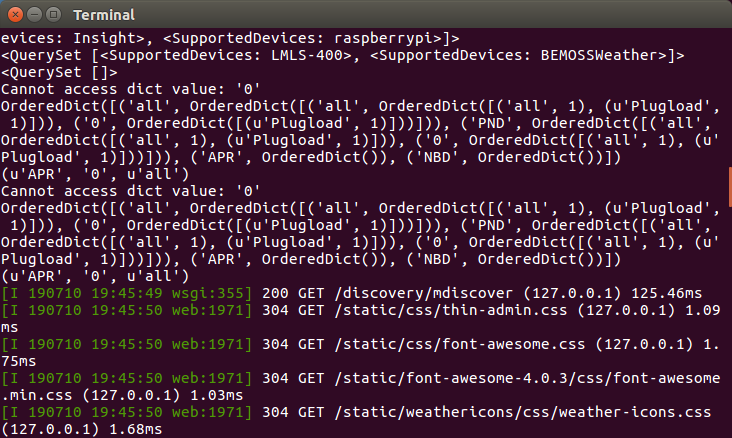
\includegraphics[scale=0.5]{figs/orderedDictError.png} 
\bigbreak\noindent
In the lab, I was able to successfully control the motor with the plugload interface by making changes to the file \texttt{API\_RaspberryPi.py}. More work was done to correct the error.

\labday{Thursday, July 11, 2019}
To test whether the new API script I wrote was the cause of the problem, I moved the file \texttt{API\_RaspberryPi.py} to the home directory and restarted BEMOSS. The message \texttt{Cannot access the value, returning default: 0} was still printed to the server log at startup, so the only thing I can conclude is that this is not an issue with the new API file. As another test, I will install BEMOSS in another directory. The same messages were printed to the log when attempting to the get the number of devices on the network, so at this point the messages will be ignored.
\bigbreak\noindent
As a first step in automating the discovery process, I added the line to the method discover in \texttt{API\_RaspberryPi.py}
\begin{verbatim}
nmap = subprocess.check_output('sudo nmap -sn 192.168.1.0/24',shell=True)
\end{verbatim}
When this line is run, a \texttt{CalledProcessError} is thrown which remove nmaps as an option that can be used to detect device information. The command was attempted to be run without superuser priviliges; however, raw IP packets are needed to resolve MAC addresses and manufacturer names with nmap.

\labday{Friday, July 12, 2019}
I completed writing the discover method for the Raspberry Pi API today. A file named \texttt{ownerinfo.json} was added to the research directory where the mac address of the Raspberry Pi used to control the motor can be added. This makes identifying the correct Raspberry Pi easier as it is possible that more than one Pi could be on the network at the same time. The command nmap was used to ping all machines on subnet 255.255.255.0. After this has been done information is stored in the machine's cache so that the address resolution protocol (arp command) may be used to find the mac addresses corresponsding to the ip address on the network. After this, it is determined whether the pi's mac addresses is located in the output of the \texttt{arp -a} command.
\bigbreak\noindent
I need to research DNS python packages to find the username of Raspberry Pi. Also, methods for storing the Raspberry Pi's password securely in the BEMOSS database must be researched.

\labday{Monday, July 16, 2019}
After doing some research I decided that I will be attempting to discover the Raspberry Pi with SSDP (Simple Service Discovery Protocol) rather than using the \texttt{nmap} and \texttt{arp} commands. Research will need to be done on these two protolocols to be able to understand how to discover and control the RPi.
\bigbreak\noindent
UPnP or Universal Plug and Play consists of three different protocols which are 
\begin{itemize}
\item SSDP (Simple Service Discovery Protocol) for finding devices on the network
\item SCPD (Service Control Point Definition) defines the actions provided 	
\item SOAP (Simple Object Access Protocol) calls actions
\end{itemize}
I found after further research that UPnP is simply not going to work with raspberry pi as it is more designed for home media servers and not suited for my specific application which is running commands on the Pi.

\labday{Tuesday, July 16, 2019}
I attempted to run the command \texttt{sudo nmap -sn 192.168.1.0/24} in the discover method; however, I was not able to login in the volttron log terminal although the prompt for the password did appear. I attempted to launch the terminal as superuser by running the command to launch the terminal in the \texttt{GUI.py} as superuser. However, I ran into several issues involving priviliges although I did remove the sudo prefix from the command. Now I will reinstall BEMOSS.
\bigbreak\noindent
Rather than using both the nmap and arp commands together I made the decision to running the nmap command as superuser to resolve the manufacturer names and MAC addresses. I ran into a problem when using \texttt{subprocess.call('sudo nmap -sn 192.168.1.0/24')} as the terminal does not allow any text to be passed to stdin while the agents are running. In addition, execution of the function will continue even though system password is provided. In the end I decided to revert back to the original code as the motivation for running nmap as super user is to retrieve the mac and IP addresses.
\bigbreak\noindent
Lastly, I found that the Raspberry Pi contains an option named Remote GPIO in the Raspi-Config which will enable the GPIO pins to be controlled over the network. No login is required to access the pins on this server only the IP address. This will hopefully streamlines tasks involving the gpio pins greatly.

\labday{Wednesday, July 17, 2019}
Following work on my presentation, I discussed with Dr. Miah using the Remote GPIO which was agreed upon. However, for the next presentation I would like to have a fully functional interface using the current method. This will require me to encrypt both the username and password of the Raspberry Pi and store in the json file that the raspberry pi API file accesses. Thus some research will need to be done on how to perform this encryption. Later (next week) I would like to get the remote GPIO interface working and implemented. Some problems still exist with this method such as security as multiple different machine may be able to control the GPIO pins at once. Also, the XBee library that is used to control the xbee modules might not be compatible with the latter method. I know very little of how zigbee communication works or how the modules work, so this will require much research.
\bigbreak\noindent
I encrypted both the username and password of the raspberry pi by using the function \texttt{encrypt\_value} in the module \texttt{bemoss\_lib.utils.encrypt} and placed both these encrypted strings in the json file. I found that I needed to decrypt the values when formatting the string used to ssh into the pi. After finding that only the password must be encrypted, I replaced the username in the json file with the plain text version.

\labday{Thursday, July 18, 2019}
Today, I found that I have not implemented the method \texttt{identifyDevice} in the Raspberry Pi API. It is to be implemented as follows:
\begin{itemize}
\item At start, \texttt{identifyDeviceResult = False}
\item Keep the current state of one of the changeable device variables (in this case the status)
\item Change device variable that is visually noticeable
\item Delay for 5 seconds
\item Change device variable back to previous state
\item if successful, \texttt{identifyDeviceResult = True}
\end{itemize}
After looking through some of the Philips Hue API code, I found that the method \texttt{get\_variable} is used to check whether the device is on or off rather than directly communicating with the device through the method \texttt{getDataFromDevice} like in the WeMo plugload API. As a test I will print \texttt{get\_variable('status')}in the method \texttt{identifyDevice} in the Raspberry Pi API to check whether this key value pair is in the dictionary defined in the BaseAPI's constructor. As of now, I do not know of a way of checking the status of the motor from the RPi using the GPIO pins and XBEE modules, so using the method from the Philips Hue API would be ideal.
\bigbreak\noindent
After pressing the button \texttt{Identify Device} in the list of plugload controllers, the message logged to the console is always \texttt{'ON'}. The reason for this is likely the code I wrote in the method \texttt{getDataFromDevice} which is shown below:
\begin{Verbatim}[tabsize=4]
def getDataFromDevice(self):
	# TODO 
	devicedata = dict()
	devicedata['status'] = BEMOSS_ONTOLOGY.STATUS.POSSIBLE_VALUES.ON 
	# setting the value to "ON"
	return devicedata
\end{Verbatim}
The statement \texttt{BEMOSS\_ONTOLOGY.STATUS.POSSIBLE\_VALUES.ON = 'ON'} is defined in the file \texttt{BEMOSS\_ONTOLOGY}. From the BEMOSS developer resources for layer 4 of the BEMOSS hierarchy I found:\\

"Out of all the above methods, the getDataFromDevice method can be periodic. This means
it can query and receive device data periodically. This ensures that the data are updated."\\

In the Basic Agent source code, a method name \texttt{deviceMonitorBehavior} is called periodically which calls \texttt{getDeviceStatus}. A call to \texttt{getDataFromDevice} occurs here which returns a dictionary and calls \texttt{convertDeviceStatus} to update the \texttt{variables} dictionary which is declared by the \texttt{BaseAPI}. Thus I must find a way to directly query the Raspberry Pi for the motor status. To start the pin mappings are between the RPi and XBee s2c module are listed below:

\begin{center}
\begin{tabular}{|c|c|}
\hline
Raspberry Pi & XBee S$2$C\\
\hline
$6$ (GND) & VSS\\
$8$ (TXD) & DIN\\
$10$ (RXD) & DOUT\\
$17$ ($3$V$3$) & VCC\\
\hline
\end{tabular}
\end{center}

\labday{Friday, July 19, 2019}
In the afternoon session with the members of ram group, I experimented with the AT commands used to control the remote XBee connected to the L$298$N H-Bridge driver. The pin mappings are shown in the table below:
\bigbreak
\begin{center}
\begin{tabular}{|c|c|}
\hline
XBee & L$298$N\\
\hline
IO$3$ & I$2$\\
\hline
IO$4$ & I$1$\\
\hline
\end{tabular}
\end{center}
\bigbreak
Also, from the L$298$N datasheet this table lists the DC motor control A pins and how the output of the h-bridge is effected:
\bigbreak
\begin{center}
\begin{tabular}{|c|c|c|c|}
\hline
EA & I$1$ & I$2$ & Motor A status\\
\hline
$0$ & $0$ & $1$ & Clockwise rotation\\
\hline
$0$ & $1$ & $0$ & Anticlockwise rotation\\
\hline
\end{tabular}
\end{center}
\bigbreak
As a side note, the EA port is used for PWM.
\bigbreak
However, the shaft rotations are swapped when using the motor in the lab.

\labday{Monday, July 22, 2019}
One of the AT commands use to read the digital IO of the XBee modules is the IC (Digital Change Detection) command. The command can "set or read the digital I/O pins to monitor  for changes in the I/O state." When the DIO state changes, a sample can be sent immediately to the coordinator XBee from the remote XBee. However, this does not send any information on the state of the pin. The command IS "forces a read of all enabled digital and analog input lines." Of course, here a wire will be need to be connected between the output pin (IO$3$ or IO$4$) and another pin configured as a digital input. When the device needs to be queried for the status of the digital IO pins, the command IS will be sent to the remote XBee. Then using the method \texttt{XBee.wait\_read\_frame} I can read the data received on the UART connection from the remote XBee. Tomorrow, in the lab this will need to be experimented with.

\labday{Tuesday, July 23, 2019}
I tried using the commands mentioned in yesterday's lab notebook to no avail. This is the code I wrote to try to receive data sent from the remote XBee:
\begin{Verbatim}[tabsize=4]
from xbee import XBee
import serial
import time

ser = serial.Serial('/dev/ttyS0',9600)
xbee = XBee(ser)

xbee.remote_at(
		dest_addr=b'\xff\xff'
		command='D3'
		parameter=b'\x04')
xbee.remote_at(
		dest_addr=b'\xff\xff'
		command='IS'
		parameter=b'\x03')
while True:
	try:
		print(xbee.wait_read_frame())
	except KeyboardInterrupt:
		break
\end{Verbatim}
The XCTU software was downloaded to work on configuring the remote MotorDriver XBee. IR, sample rate, was set to 1000 ms or a hex value of 0x3e8 and D1, dio1, was set as a digital input. Running \texttt{ser.read()} results in an output of \texttt{'\textbackslash x00'}. Thus, no data is being received even though data should be sent to coordinator at a rate of 1 second.

\labday{Wednesday, July 24, 2019}
I decided to try experimenting with the digi-xbee python library. After following the instructions to configure the devices at 

\url{https://xbplib.readthedocs.io/en/latest/getting_started_with_xbee_python_library.html#gsginstall},
I was unable to send AT commands to the end point XBee to toggle the motor. This was later resolved after setting the output values of IO$3$ and IO$4$ to opposite values using XCTU. Later I was able to read the digital values of these IO lines (whether they are high or low). This means that only two IO lines will be needed to control the remote XBee module rather than 4 as the status of the IO line can be read directly even if it is a digial output. A script was written named \texttt{XBEEcontrol.py} that can toggle the motor and determine the status of the enabled pins on the remote XBEE. At the end of the day I was able to successfully identify the motor by toggling it twice with a 5 second pause inbetween. The last part of the implementation is adding the motor images to the frontend.

\labday{Thursday, July 25, 2019}
I found an picture of the GM$8000$ series motor and added images denoting when the motor is on and off to the \texttt{Web\_Server/static/images} directory after removing the default background with GIMP.
\bigbreak\noindent
The next task is working on adding a new device type to BEMOSS called 'Motor'. In the file \texttt{Web\_Server/run/defaultDB.py}, I added the lines
\begin{verbatim}
dt5 = DeviceType(id=5, device_type='Motor')
dt5.save()
\end{verbatim}

\labday{Friday, July 26, 2019}
Starting BEMOSS with changing the lines from yesterday result in an error when attempting to add the Raspberry Pi API to the list of the supported devices. After running the file \texttt{BEMOSS3.5/Web\_Server/run/defaultDB.py} by typing \texttt{python Web\_Server/run/defaultDB.py} in the \texttt{BEMOSS3.5} directory the problem was fixed. BEMOSS was started successfully; however, the widget listing Motors was not available on the 'Discover New Devices' page. In the file \texttt{Web\_Server/webapps/discovery/views.py}, on line 58, \texttt{power\_meters} was changed to motors and on line 71, the key value pair for the power\_meters in the \texttt{devices} dictionary was removed and a key value pair for motor was added. After making further changes to the javascript and html manual discovery files, the issue was not corrected. It was later found that a closing div tag was missing from the file to close the div with class "row". Another exception was thrown when trying to access the pass usage statistics.

\labday{Monday, July 29, 2019}
The following error was thrown when running the \texttt{platform\_initiator.py} file when attempting to add the motor API to the database.
\begin{verbatim}
insert or update on table "supported_devices" 
violates foreign key constraint
"supported_devices_device_type_id_1f8832cb_fk_device_type_id"
DETAIL:  Key (device_type_id)=(5) is not present 
in table "device_type".
\end{verbatim}
This error is fixed by running the file \texttt{Web\_Server/run/defaultDB.py} which will update the BEMOSS database. Next to help clear up the VOLTTRON log file I attempted to dissect the error message reported by the Time Series Database Agent. This error is presented below
\begin{Verbatim}[tabsize=4]
Traceback (most recent call last):
	File "/usr/lib/python2.7/logging/__init__.py", line 861, in emit
		msg = self.format(record)
	File "/usr/lib/python2.7/logging/__init__.py", line 734, in format
		return fmt.format(record)
	File "/home/ramgroup/BEMOSS3.5/volttron/platform/agent/utils.py", line 242, in format
		return jsonapi.dumps(dct)
	File "/home/ramgroup/BEMOSS3.5/env/local/lib/python2.7/
	site-packages/zmq/utils/jsonapi.py", line 40, in dumps
		s = jsonmod.dumps(o, **kwargs)
	File "/home/ramgroup/BEMOSS3.5/env/local/lib/python2.7/
	site-packages/simplejson/__init__.py", line 399, in dumps
		**kw).encode(obj)
	File "/home/ramgroup/BEMOSS3.5/env/local/lib/python2.7/
	site-packages/simplejson/encoder.py", line 296, in encode
		chunk = self.iterencode(o, _one_shot=True)
	File "/home/ramgroup/BEMOSS3.5/env/local/lib/python2.7/
	site-packages/simplejson/encoder.py", line 378, in iterencode
		return _iterencode(o, 0)
	File "/home/ramgroup/BEMOSS3.5/env/local/lib/python2.7/
	site-packages/simplejson/encoder.py", line 273, in default
		o.__class__.__name__)
TypeError: Object of type DefaultEndPoint is not JSON serializable
Logged from file connection.py, line 1100
\end{Verbatim}
A logging issue is obviously present here and these stack traces are printed via logging message. Logging messages can have different levels of severity. In increasing order they are:
\begin{itemize}
\item DEBUG: Detailed information, typically of interest only when diagnosing problems.
\item INFO: Confirmation that things are working as expected.
\item WARNING: An indication that something unexpected happened, or indicative of some problem in the near future (e.g. ‘disk space low’). The software is still working as expected.
\item ERROR: Due to a more serious problem, the software has not been able to perform some function.
\item CRITICAL: A serious error, indicating that the program itself may be unable to continue running.
\end{itemize}
The error above has level ERROR so the TSD Agent is not able to perform some function.
\bigbreak\noindent
It appears as if some objects cannot serialized by the python json module after some investigation. A possible fix to this problem is removing all the debug logging statements from the files in the cassandra python driver. However, this would take a great deal of time as there are many of them. Also, these logging statements are likely needed in case another problem arises. As mentioned from the log statements, on line \texttt{1100} of \texttt{cassandra.connection.py}, the following debug log statement exists:
\begin{verbatim}
log.debug("Sending options message heartbeat on idle connection (%s) %s",
                 id(connection), connection.endpoint)
\end{verbatim}

\labday{Tuesday, July 30, 2019}
In the lab, I found that the verision of the Datastax python driver used by the previous senior project group is different and only logs host names to the file rather than objects of classes defined inside the connection file. Today, I will meet with Dr. Miah to work on resolving this issue. While working on testing the motor interface I found that the power supply is not working properly. It fails to turn on immediately when the \texttt{XBEEcontrol.py} script is run with the argument \texttt{turnOnMotor}. A potential cause is the lack of a flyback diode across the input terminals to the motor which could be damaging the power supply due to voltage spikes.

In the meantime, before the meeting, I will work on trying to add plugload chart onto the motor page. Even though I am able to control the motor with the switch and identify device button, none of the data is added to the database. Something to note is that each table in BEMOSS is named according to the \texttt{agent\_id}. Somewhere in the repository these tables are added to the database; however, it is unclear where that occurs. According to the BEMOSS-Data-Management section of the developer resources: "During operation, the device agents connect to the Cassandra node on the same machine the agent is running, using Cassandra python driver, and writes time series data to a unique table named after the device\_id it is controlling."

After the meeting with Dr. Miah, it was determined that the current bug involving the cassandra python driver is a top priority. No paper will be submitted if this current issue still exists. A print statement was added on lines $133$ and $139$ of the TSDAgent source code: \texttt{print(message)}. One of the messages logged to the \texttt{volttron.log} file is 
\begin{verbatim}
{u'tablename': u'platform_event', u'all_vars': 
{u'event_id': u'155df44e-e45b-4271-bc44-ce053509d22a', u'start_time': 
u'2019-07-31 04:37:42:936113*None', u'date_id': u'2019-07-30', u'agent_id': 
u'platformmonitoragent_Node1', u'end_time': u'2019-07-31 
04:38:44:552121*None'}, u'log_vars': 
{u'event_id': u'UUID', u'start_time': u'TIMESTAMP', u'date_id': u'text', 
u'agent_id': u'text', u'end_time': u'TIMESTAMP'}}
\end{verbatim}
 
\labday{Wednesday, July 31, 2019}
This morning I checked the version of the cassandra-driver for python on the current machine. It is $3.18.0$ and the version on Bob's machine is $3.16.0.$ Also, after commenting out lines $135$ and $141$ in \texttt{Agents/TSDAgent/TSD/agent.py}, the same logging error was reported to the volttron log file. Thus, the function \texttt{do\_insertion\_jobs} is not the only problem rather also the \texttt{insert} and \texttt{customInsert} functions. In all, the cause of this problem will be very difficult to find as there are likely many calls to methods in the cassandra-driver package. In addition, another error is reported involving the VOLTTRON bacnet proxy agent when my machine is connected to both Wi-Fi and Ethernet. This problem is resolved if the host computer is only connected to the ECE-Robotics 1 network when running BEMOSS. A screencap is posted below.
\begin{figure}[h]
\center
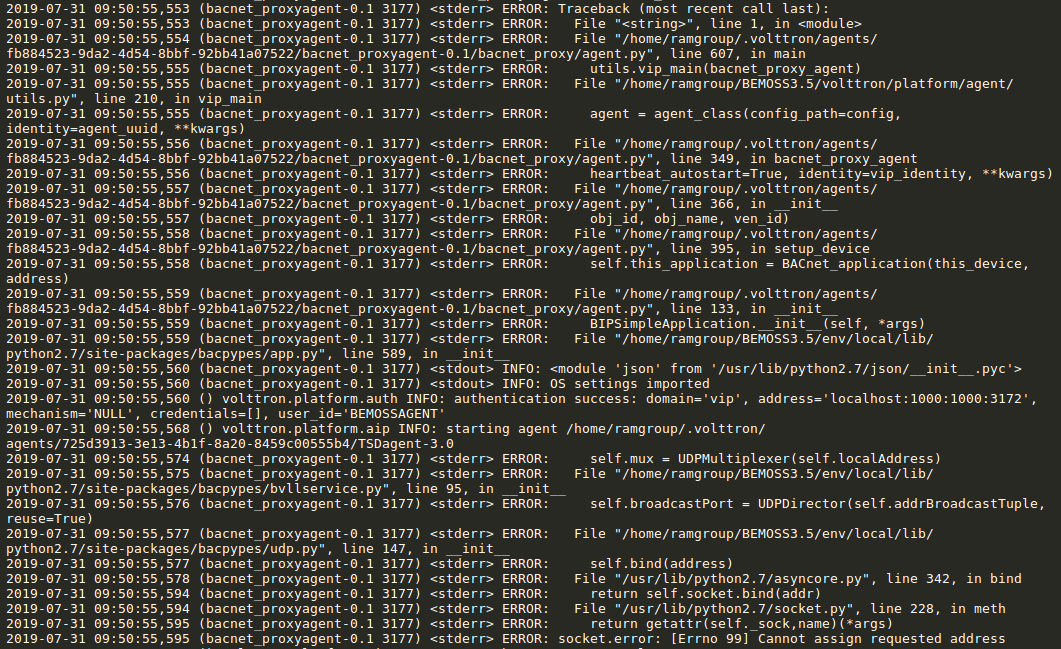
\includegraphics[scale=0.3]{figs/bacnetAgentError.png}
\end{figure}
A attempt to correct the error was made by cloning BEMOSS into a new repository and ensuring the version $3.16.0$ was installed rather than the latest $3.18.0$. Next time, however, I need to dig deeper into the issue and understand it rather than use the "hack it until it works method". Due to time constraints, I used this method instead. The TSD agent errors were no longer present; however, another possible unrelated error was thrown by the network agent:
\begin{Verbatim}[tabsize=4]
Traceback (most recent call last):
  File "/home/ramgroup/tests/BEMOSS3.5/volttron/platform/
  vip/agent/subsystems/rpc.py", line 168, in method
    return method(*args, **kwargs)
  File "/home/ramgroup/tests/BEMOSS3.5/volttron/platform/vip/
  agent/subsystems/pubsub.py", line 262, in _peer_push
    callback(peer, sender, bus, topic, headers, message)
  File "/home/ramgroup/.volttron/agents/
  90ab11e3-bdb4-45e7-95c7-c3cbf682b92b/networkagent-0.1/network/agent.py", 
  line 222, in on_match_change
    self.curcon.commit()
  File "/home/ramgroup/tests/BEMOSS3.5/
  bemoss_lib/utils/db_helper.py", line 82, in reconnect
    return func(*args,**kwargs)
  File "/home/ramgroup/tests/BEMOSS3.5/
  bemoss_lib/utils/db_helper.py", line 109, in commit
    return self.con.commit()
IntegrityError: insert or update on table "node_device" 
violates foreign key constraint 
"node_device_assigned_node_id_cba9785e_fk_node_info_node_id"
DETAIL:  Key (assigned_node_id)=(0) is not present 
in table "node_info"
\end{Verbatim}
Unfortunately, as time went on the errors involving the TSD agent appeared again. At this point I have very little idea what is causing the issue. I do have a theory that the replaced URL is causing problems. So I will run a few tests:
\begin{enumerate}
\item Run BEMOSS with resource from old link (\texttt{dsc-cassandra-3.0.9-bin.tar.gz}) with cassandra-driver $3.16.0$ on ramgroup laptop
\item Run BEMOSS with resource from old link (\texttt{dsc-cassandra-3.0.9-bin.tar.gz}) with cassandra-driver $3.18.0$ on ramgroup laptop
\end{enumerate}
Number 1 could not be done as the cassandra directory cannot simply be transferred from one BEMOSS directory to another when installing. After performing 2, the same TSD agent errors occurred leading me to strongly believe that this has something to do with the python cassandra driver. I will run BEMOSS again with the new link and cassandra-driver $3.16.0$. The version of the cassandra-driver packaged is changed with the command \texttt{pip install cassandra-driver==version} after running the command \texttt{. env/bin/activate} to run the previous command in the BEMOSS virtual environment. After further testing I found that errors will be thrown by the time-series database agent with the cassandra-driver $3.16.0$ only when BEMOSS run is run for the first time. 
\end{addmargin}

%----------------------------------------------------------------------------------------
%	BIBLIOGRAPHY
%----------------------------------------------------------------------------------------


\bibliographystyle{plain}
\bibliography{bib/seniorProject2017.bib}


% \begin{thebibliography}{9}

% \bibitem{lamport94}
% Leslie Lamport,
% \emph{\LaTeX: A Document Preparation System}.
% Addison Wesley, Massachusetts,
% 2nd Edition,
% 1994.

% \end{thebibliography}

%----------------------------------------------------------------------------------------

\end{document}


%%% Local Variables:
%%% mode: latex
%%% TeX-master: t
%%% End